In this section we will illustrate the qualification process for the
openETCS tool chain.
As an example we will focus on the sample tool cahin depicted figure
\ref{fig:sample}

\begin{figure}[h]
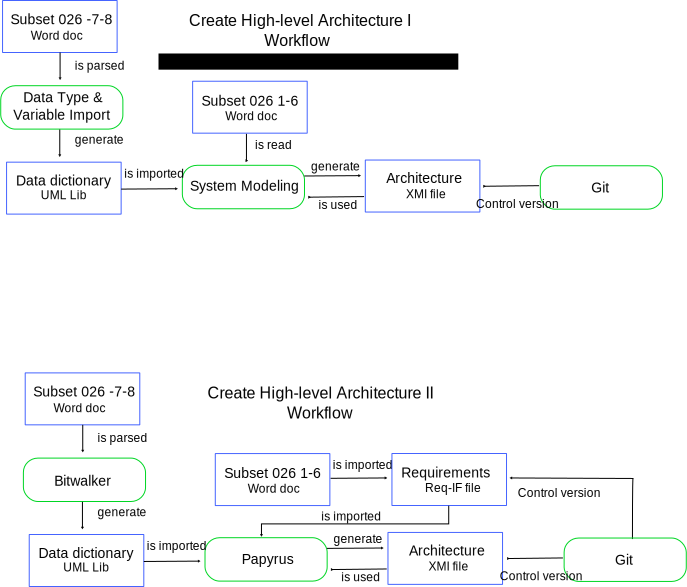
\includegraphics[width=\textwidth]{toolchainsample}
\caption{\label{fig:sample} Tool chain samples} 
\end{figure}

The first tool chain : Create High-level Architecture I proposes to
create a high level view of the on board unit from the Subset 026
specification. It  is composed by
two features.  
\subsection{Qualification process for tool chain I}
\paragraph{Step 1: Feature Analysis}
{\bf Feature 1: Data type and Variable Import}\\
\begin{description}
\item Tool 1: Bitwalker 
  \begin{itemize}
  \item Tool Identification: Bitwalker v1.0
  \item Tool Origin: Self-developed
  \item Tool license: EUPL
  \item Tool Justification: 
  \item Tool Input/Output: 
  \item Tool dependencies: None
  \item Use cases:
  \item Tool Class: T3
  \item Potential errors: see \ref{sec:bitwalker-example}
  \item How to Provide Evidence: see \ref{sec:bitwalker-example}
   \end{itemize}
\item Tool 2: Data Dictionary
\begin{itemize}
  \item Tool Identification: Data Dictionary  based on SRS 0.1.201407031006
  \item Tool Origin: Self-developed
  \item Tool license: EUPL
  \item Tool Justification: 
  \item Tool Input/Output: 
  \item Tool dependencies: None
  \item Use cases:
  \item Tool Class: T3
  \item Potential errors: 
  \item How to Provide Evidence:
   \end{itemize}
\end{description}

{\bf Feature 2: System Modeling}\\
  \begin{itemize}
  \item Tool Identification: Papyrus  0.10.1.v20130918
  \item Tool Origin: Eclipse Incubation (CEA)
  \item Tool license:  
  \item Tool Justification: Papyrus is a modeling tool that allows us
    to model the high-level architecture of the OBU with SysML.
  \item Tool Input/Output: 
  \item Tool dependencies: 
  \item Use cases:
  \item Tool Class: T3
  \item Potential errors:
  \item How to Provide Evidence:                 
  \end{itemize}

{\bf Feature 3: Artifacts Versioning}\\
  \begin{itemize}
  \item Tool Identification: Eclipse  Egit   3.2.0.2013121812
  \item Tool Origin: Eclipse foundation
  \item Tool license:  Eclipse Public License Version 1.0
  \item Tool Justification: Egit provides an implementation of the Git
    version system. 
  \item Tool Input/Output: 
  \item Tool dependencies: JGit Core
  \item Use cases:
  \item Tool Class: T2
  \item Potential errors:
  \item How to Provide Evidence:                 
  \end{itemize}


\paragraph{Tool platform Analysis}
This should only be T1 feature ?
\begin{itemize}
\item List of services in Use : GUI ...
\item Version Compatibility
\end{itemize}
\paragraph{Tool chain Analysis}
\begin{itemize}
\item Tool dependency Analysis: All tool needed present with a
  compatible version (Need a matrix)
\item Tool Artifacts interaction matrix: Use for compatibility format
  and to highlight interactions
\item List of new Potential error due to interaction
\item How to provide evidence 
\end{itemize}

\subsection{Qualification process for tool chain II}
How to process changes, the different possible change within the tool
chain are add, update, replace or remove a tool.

